\subsection{Control Module}
\subsubsection{Design Procedure}
The Control Module is the brain of the system, where all the processing and decision-making occurs. It is responsible for receiving input from the user, processing that input, and sending commands to the Actuator Module. The core of the control module is the Unity, it received the control signal from VR handler, like pressing the buttons to move the UR3 arm and the grip process of claw, then, it translate command signal to the parameters of motor and sent it to subcontrollers. 
  
In addition to Unity, we added a STM32 board to control the stepper motor to finish the closed-loop control of claw, inorder to ensure the stability of grisping. After confirming the main controllers in module, I need to think about how to connect them with each other or other modules. Through refering to the ST company manual of STM407ZG chip, I found that it supports the USART communication protocol, which means it can receive the command from PC Unity with UART line. Moreover, it also has pins with CAN\_RX and CAN\_TX, which also supports me to control the stepper motor with CAN protocol ~\cite{stm32f407zg}. 
  
After designing the flow path, I wanted to add a sensor on claw to monitor the grip power, so I added the FSR402 pressure sensor and connect it to STM board. Overall, I got the main data flow idea.
  
\subsubsection{Design Details}
Aftering determining the main data flow theorically, I design to set up hardware circuit, therefore, I drew the design graph, as shown in the Figure \ref{fig:design_circuit}. This introduces the main connection of control module.
\newpage
\begin{figure}[h]
    \centering
    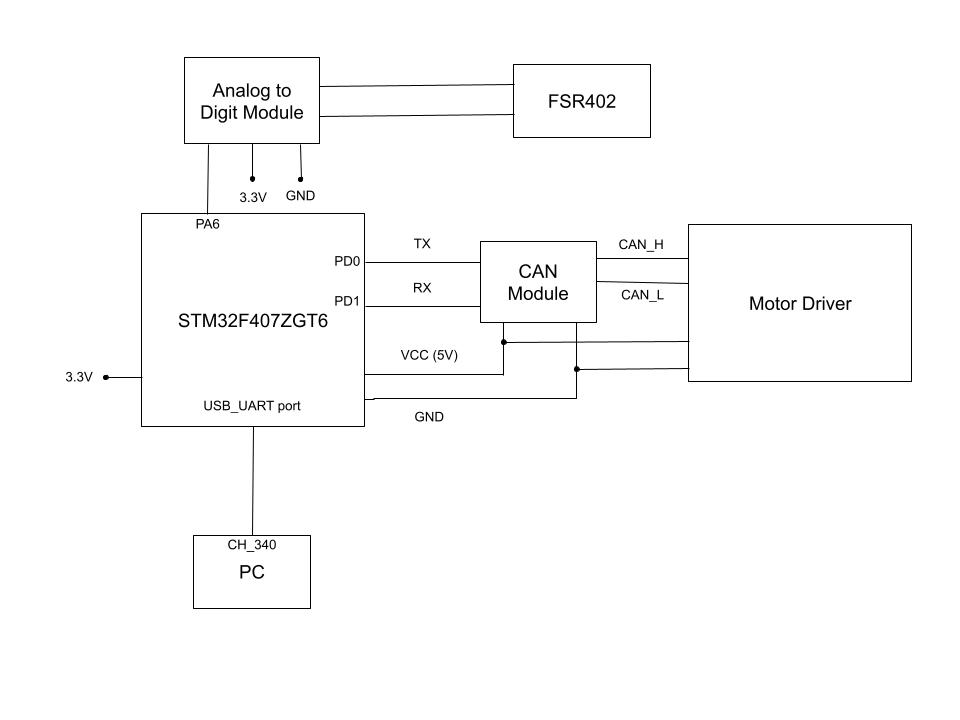
\includegraphics[width=0.8\textwidth]{Figures/Design Circuit.jpg}
    \caption{Design Circuit}
    \label{fig:design_circuit}
\end{figure}
  
\textbf{CAN Communication:} 
  
Through referring to the motor driver board X42\_V1.3 instruction manual, it allows us to use intergrated CAN command to control the stepper \cite{zhang2023csdn}. However, the STM32F407ZG only have RX and TX pins, the transmition of CAN signal should be CAN\_H and CAN\_L two logical voltage \cite{liu2024csdn}, which means I need to design a CAN receive and send message module. After searching online, I decided to use the TJA1050 chip to convert the digital CAN signals from the microcontroller to the differential voltage signals required by the CAN bus and vice versa, as shown in the figure~\ref{fig:can_module}.
The TJA1050 is a CAN transceiver IC that acts as a bridge between the CAN controller (STM32) and the physical CAN bus. It converts single-ended digital signals from the microcontroller into differential signals suitable for transmission over the CAN network, ensuring noise immunity and reliable data communication. At the receiving end, it converts the differential bus signals back into digital signals that can be interpreted by the microcontroller. And to ensure that the bus signals are stable, two 120 $\Omega$ resistors should be connected in parallel at both ends of the CAN bus~\cite{liu2024csdn}.
\begin{figure}[h]
    \centering
    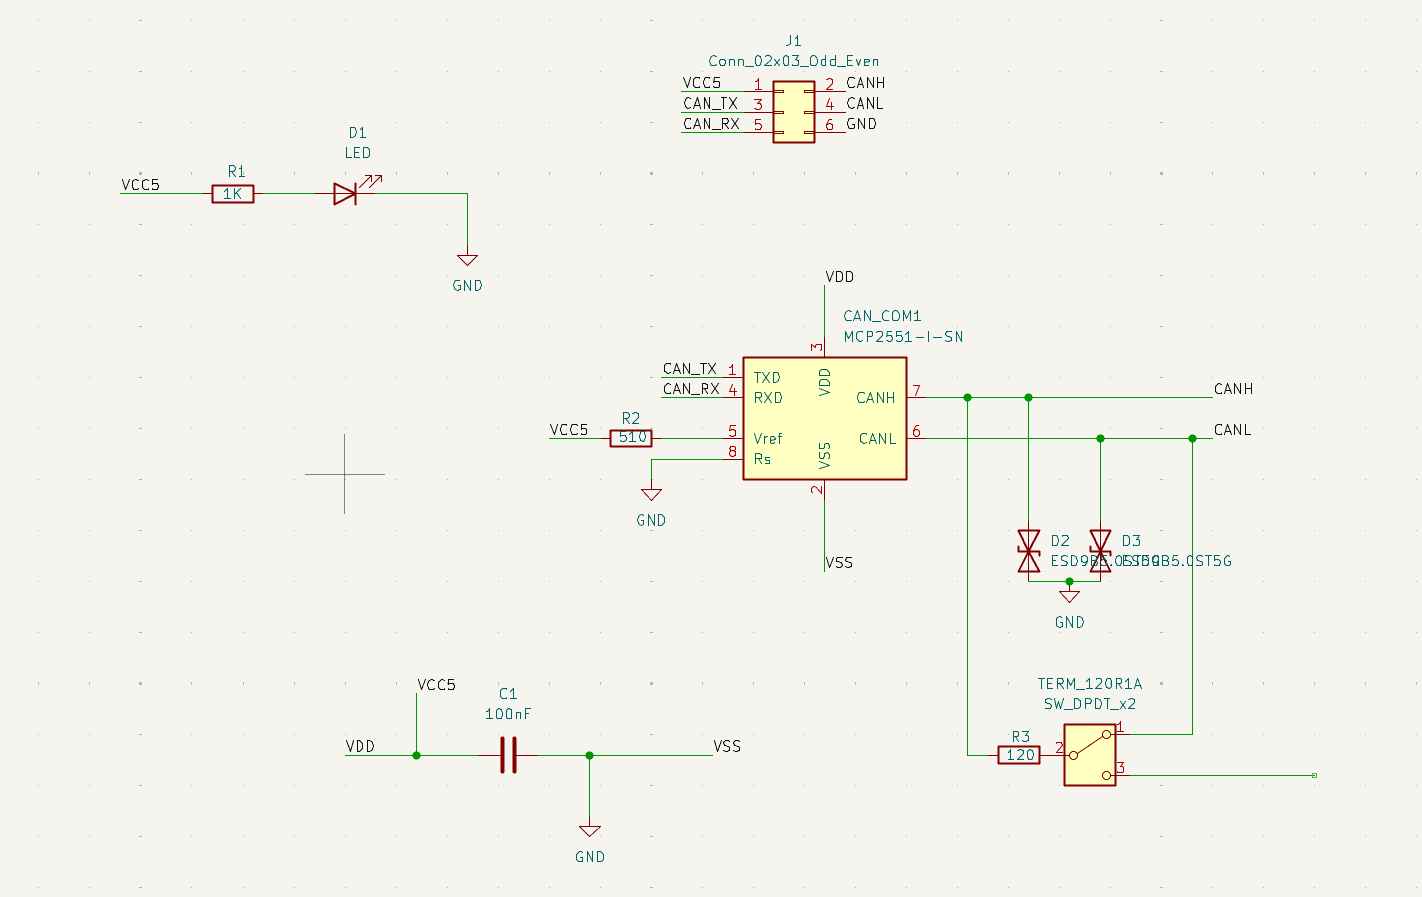
\includegraphics[width=0.8\textwidth]{Figures/CAN_MODULE.png}
    \caption{CAN Module}
    \label{fig:can_module}
\end{figure}
  
\textbf{Pressure Sensor:} 
  
The FSR402 pressure sensor is a force-sensitive resistor that changes its resistance based on the amount of force applied to it. It is commonly used in applications where measuring pressure or force is required. The FSR402 sensor works by changing its resistance when a force is applied to its surface. The more force applied, the lower the resistance. By measuring the voltage across the sensor, we can determine the amount of force being applied. I develop two approaches to read the sensor data: 
\begin{enumerate}
    \item Using the default ADC (Analog-to-Digital) port of STM32F407ZG, which is a 12-bit ADC. The ADC converts the analog voltage signal from the FSR402 into a digital value that can be processed by the microcontroller. The ADC can be configured to read the voltage across the sensor and convert it into a corresponding digital value. 
    \item Using the LM393 chip to compare the voltage on pressure sensor with referrence voltage (Variable Resistance). When the voltage on FSR402 is larger than referrence, the output will be high voltage. When the pressure is larger than desired, it will change voltage, which achieves simple Analog to Digita transform. 
\end{enumerate} 
For convinient, I design a circuit intergrated on a small PCB~\ref{fig:fsr402_pcb} and soldering it. The circuit is shown as Figure~\ref{fig:fsr402_circuit}. In circuit, I connect the FSR402 with 10k$\Omega$ resistor. AO port will output the voltage on FSR402 under 3.3V input, using for the $1{st}$ method. DO port with output the compare consequence of FSR voltage and 10k $\Omega$ variable resistance voltage, using as GPIO input for 2ed method. Finally, I decide to use the $2^{ed}$ method and the reson will be explained in Verification and Test part.
\begin{figure}[h]
    \centering
    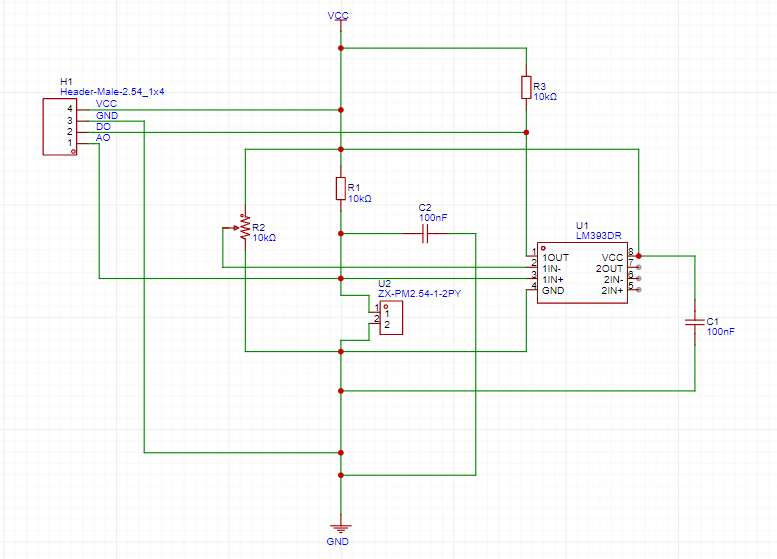
\includegraphics[width=0.8\textwidth]{Figures/FSR402_CIR.png}
    \caption{FSR402 Circuit}
    \label{fig:fsr402_circuit}
\end{figure}
  
\textbf{Coding Explain:}
  
Coding in control module is a huge and most complex part, I will introduce it with two aspects: STM32 and Unity.
  
In STM32, I develop the codes based on the HAL library which is configured by STM32CubeMX and implemented them in KDM5 (Keil Development Environment).
\begin{itemize}
    \item \textbf{can.c:} 
    The HAL (Hardware Abstraction Layer) library provides a high-level interface for configuring and using the CAN peripheral. What I did is initializing the handler and change the can\_send() function to send standard CAN message to tell the 42 stepper to run its position circle, like move to which position, how fast, when stop, and so on. In addition, I also need to write the receive function to receive the position feedback of motor to control its stop time. For example, if I send 01 36 6B to request the position of motor, it will response 01 36 01 00 01 00 00 6B, which means the postion is 0x00010000 (16), direction is positive. The send function runs smoothly, but the feedback function costs me plenty of time to debug.
    \item \textbf{usart.c:}
    The UART (Universal Asynchronous Receiver-Transmitter) peripheral is used for serial communication with the Unity application. The HAL library provides functions to initialize the UART peripheral and rewrite the HAL\_UART\_RxCpltCallback() function to achieve the communication between STM32 and Unity.
    \item \textbf{sensor.c:} 
    AsI mentioned before, I choose to use the DO as output of the pressure sensor. To achieve this, I just initialized the GPIN\_IN and open the clock of corresponding pin RCC to receive the digital signal from DO.
    \item \textbf{main.c:}
    The main function initializes the system clock, can port, uart port, sensor, and so on. After initialization, I develop the logic of gripping and releasing an infinite loop. In the loop, it continuously checks for incoming data from Unity via UART, the Unity will send "S" for start, "R" for release and "H" for stop. After receiving the start, CAN message will be send to tell motor to begin until the reflected pressure sensor data shows the claw have griped the item. When pressure is over the threshold (input low voltage change), STM32 will send CAN message to stop motor. While Unity sending release signal, the motor will return according to the position feedback minitoring. Then, the STM32 will wait for next command from Unity. The following Moore FSM(Figure~\ref{fig:motor_fsm}) shows the overall logics.
\end{itemize}
\begin{figure}[h]
    \centering
    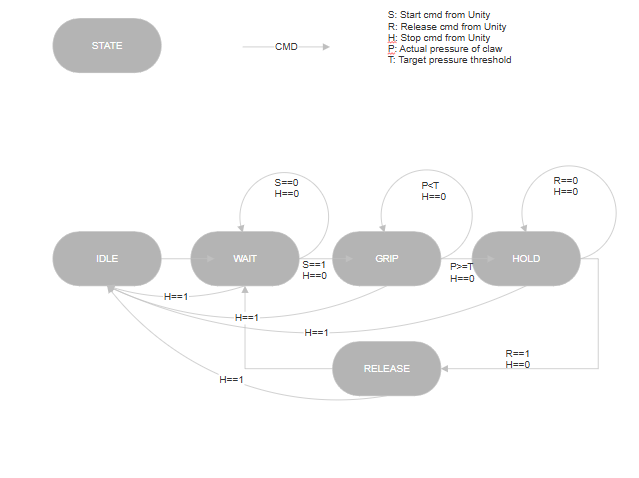
\includegraphics[width=0.8\textwidth]{Figures/SVM.png}
    \caption{Motor FSM}
    \label{fig:motor_fsm}
\end{figure}
\textbf{Unity:} 
\begin{itemize}
    \item \textbf{VR Handler:} 
    
    \item \textbf{Motor Control:} 
    
    \item \textbf{Serial Port:}
    The serial port communication in Unity is implemented using the System.IO.Ports namespace. This allows Unity to open a serial port, send data to the STM32, and receive data back. The serial port settings, such as baud rate and parity, are configured to match those of the STM32. For this project, I use the UART line to connect them and my baud rate was set in STM to 115200, therefore, the serial port in unity setting is corresponding to baud rate and use COM4 CH340 PC port.
\end{itemize}
\subsubsection{Verification and Testing}
After going through all the procedures above, I successfully set up the control module with hardware as shown in Figure~. However, I encountered plenty of problems during the testing and debugging process.
\begin{itemize}
    \item \textbf{PCB Testing:}Before the circuit above, I have designed a failed circuit, which is shown as Figure~\ref{fig:fsr402_failed_circuit}. However, I found errors after the soldering. While applying 3.3V on VCC port, the voltage on AO didn't change with the pressure on FSR402. Therefoe, I used the multimeter to check the circuit. There are errors, like the voltage on AO before FSR insertion should be 0.3V, but I measured 3.17V. In addition, resistance between VCC and DO should be $909.1\Omega$, but actually wired $9.792k\Omega$. Finally, I found there is open circuit in PCB design. Aftering designing new circuit, I succeed. The following Table~\ref{tab:pcb_testing} shows my measure history.
    \item \textbf{Baud Rate Mismatch:} While sending the CAN message (position circuit control) to the stepper motor, the motor cannot run correctly as desired. After checking the CAN related codes, I didn't find the bug. Then, I use oscillograph to check the CAN\_H port. Normally, if the CAN message send correctly, the CAN\_H will have voltage changed, the low voltage should be about 0 and high should be 5V. However, I found that the CAN\_H wave always 4.176mV, which means the CAN initialization failed. So I check the default CAN HAL init, the baud rate is set to 1M, which is mismatched from my motor's CAN receive rate. My designed baud rate should be 50000. The CAN bus baud rate on STM32 is determined by configuring the CAN timing registers, primarily the Prescaler, BS1, BS2, and SJW parameters, and the rate computation should use the equation:
    \begin{equation}
        \text{Baud Rate} = \frac{\text{CAN Clock Frequency}}{\text{Prescaler} \times (1+\text{BS1} + \text{BS2})}
    \end{equation}
    For my project, system clock is 168Mhz, the CLK OF CAN is APB1 CLK  $=\frac{\text{System Clock}}{4}=42Mhz$ I changed the Prescaler to 14, BS1 to 4, BS2 to 1. Therefore my designed baud rate should be  $\frac{42Mhz}{\text{14} \times (1+4+1)}=50000$ , which matched the default rate. After changing the baud rate, I successfully finished the communication with motor.
    \item \textbf{STM32 ADC Delay:}After comparing my two methods prepared to monitor the pressure by FSR, I found that the DO port responses the pressuree threshold faster compared with AO after ADC. I thought the DO will enable my claw more sensitive, but actually, the ADC delay is about 1ms, which is not acceptable for my project. Therefore, I choose to use the DO port as input.
    \item \textbf{CAN Feedback:}At first, I didn't think the position feedback of motor is necessary. However, I found that there are errors in phase of motor D axle, various from $0.9^\circ$ to $1.2^\circ$. With accumulation, the origin position of claw will be changed, causing the claw cannot close completely. Therefore, I added the CAN feedback function to monitor the position of axle, ensuring the motor run back until the position is 0. Through testing, the average position error decreased, within $0.08^\circ$. 
\end{itemize}


